\newpage
\section{Implementação da Metodologia RAG}

A etapa de recuperação consiste em trazer os documentos mais relevantes de acordo com a consulta ou contexto de entrada. Para alcançar isso, os documentos podem ser previamente ranqueados com base em \textit{query} de entrada ou pelo contexto específico. Essa abordagem assegura que os documentos mais pertinentes sejam priorizados e apresentados ao usuário, melhorando a eficácia e a precisão do sistema de recuperação de informações.

\subsection{\textit{Retrieval}}

A recuperação de informações pode ser realizada de duas formas principais: baseada em \textit{embeddings} de modelos e usando algoritmos tradicionais de recuperação. A recuperação baseada em \textit{embeddings} utiliza modelos de linguagem pré-treinados, como BERT ou SentenceTransformers, para gerar representações vetoriais dos textos, capturando seu significado semântico. Isso permite recuperar informações relevantes mesmo quando não há correspondência exata de palavras, mas exige mais recursos computacionais e pode ser mais lenta. Em contraste, os algoritmos tradicionais de recuperação, como TF-IDF e BM25, dependem de correspondências exatas de palavras-chave e índices invertidos, proporcionando buscas rápidas e eficientes, porém com menor capacidade de entender sinônimos e variações linguísticas. 

\subsubsection {Recuperação baseada em \textit{Modelos de Embedding}}

A recuperação de informações baseada em \textit{embeddings} se fundamenta na representação vetorial de palavras e frases. Modelos como BERT \textit{(\textit{Bidirectional Encoder Representations from Transformers})} \cite{DBLP:journals/corr/abs-1810-04805} utilizam redes neurais profundas para gerar embeddings que capturam as nuances semânticas dos textos. Esses modelos são treinados em grandes corpora de texto para aprender representações contextuais das palavras. Ao invés de comparar palavras exatas, os \textit{embeddings} permitem a comparação de vetores que representam o significado semântico, o que melhora a precisão da recuperação de informações \cite{alaparthi2020bidirectionalencoderrepresentationstransformers}. 

Na Figura \ref{fig:retrieval1} é representado o fluxo de recuperação da informação baseado em \textit{Embedding Model}.

\begin{figure}[H]
    \centering
    \caption{Recuperação baseada em \textit{Modelos de Embedding}.}
    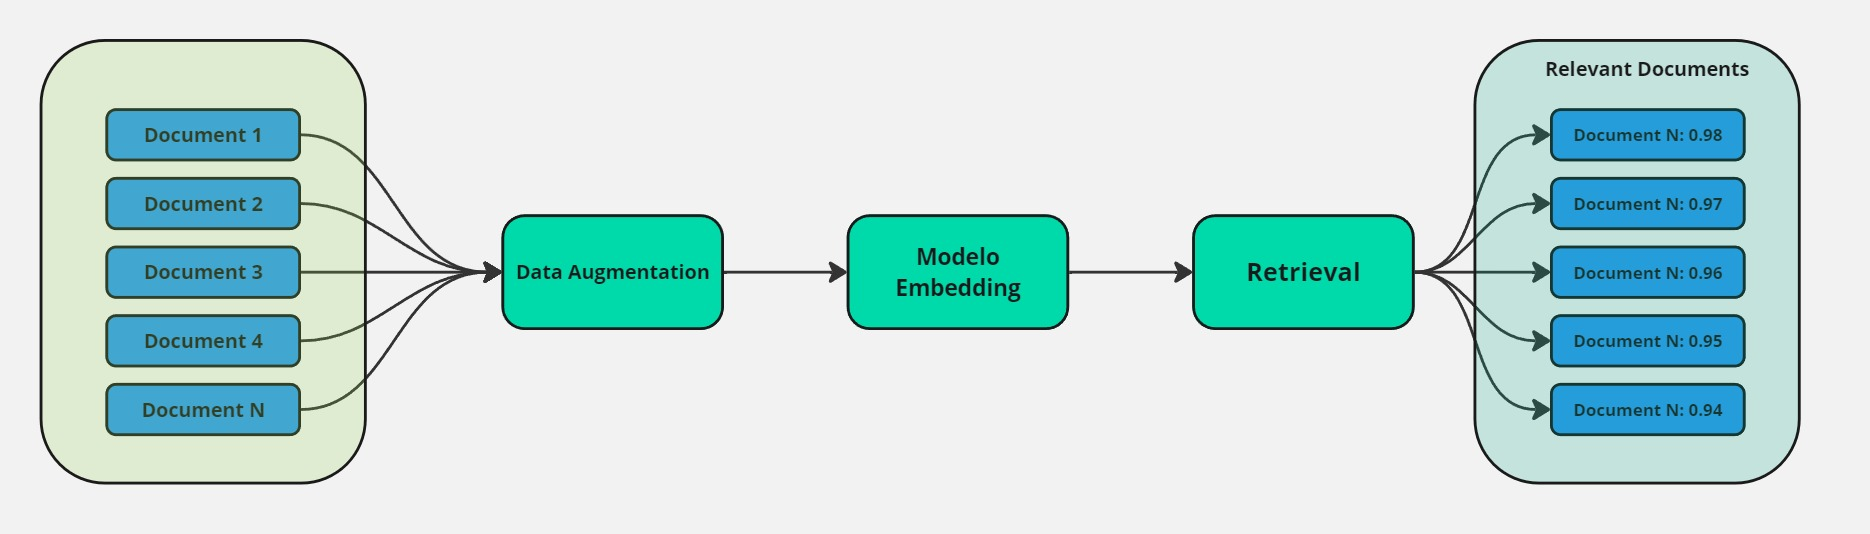
\includegraphics[width=\linewidth]{img/RAG/rag6.jpg}
    \caption*{ Fonte: Do Autor}
    \label{fig:retrieval1}
\end{figure}

\subsubsection {Recuperação baseada em algoritmos tradicionais}


Os algoritmos tradicionais de recuperação, como TF-IDF e BM25 \cite{askari2023injecting}, são conhecidos por sua eficiência e simplicidade. Eles são rápidos e eficientes em termos de tempo e recursos computacionais, facilitando a implementação sem a necessidade de treinamento de modelos complexos. A baixa latência é uma vantagem significativa desses métodos, graças ao uso de indexação invertida e outras técnicas otimizadas. No entanto, esses algoritmos apresentam desvantagens notáveis, como a falta de compreensão semântica, pois dependem de correspondências exatas de palavras, o que pode resultar em resultados menos relevantes quando as palavras exatas não estão presentes nos documentos. Além disso, são limitados a palavras-chave, dificultando o tratamento de sinônimos ou variações linguísticas, e são menos flexíveis, exigindo ajustes significativos para serem adaptados a diferentes domínios e contextos.


\subsubsection{Normalização}

A limpeza de dados é um passo crucial na geração de embeddings, tanto em modelos pré-treinados para \textit{fine tuning} quanto em algoritmos tradicionais de ranqueamento. Dados de qualidade garantem que os \textit{embeddings} capturem com precisão as nuances semânticas do texto, melhorando a eficácia do modelo. Isso inclui a remoção de ruídos como caracteres especiais, normalização de texto (convertendo tudo para minúsculas), remoção de \textit{stopwords} (Stopwords são palavras comuns que são removidas no processamento de texto porque não adicionam significado significativo. Exemplos incluem "o", "a", "e", "de".), e tratamento de valores ausentes ou duplicados. Em modelos de \textit{fine tuning}, uma limpeza rigorosa dos dados assegura que o modelo se adapta corretamente ao domínio específico, evitando viéses e garantindo representações precisas. Da mesma forma, em algoritmos de ranqueamento, dados limpos são essenciais para criar índices eficientes e realizar buscas precisas, maximizando a relevância dos resultados retornados.

Com isso, os passos fundamentais para garantir a qualidade de dados é dada pelos seguintes fatores:
\begin{itemize}
    \item Remoção de \textit{stopwords}
    \item Remoção de tags de HTML.
    \item Remoção de caracteres especiais. 
    \item Remoção de acentuação.
    \item Lematização das palavras. Por exemplo: "Correndo", "correu", se transformará em "Correr"
    \item Transformação para palavras minúsculas. Como "Correr" se transformará em "correr".
\end{itemize}



\subsubsection{Tokenização}

A tokenização é o processo de segmentar um texto em unidades menores, chamadas tokens, que podem ser palavras, caracteres ou frases, dependendo do contexto e do objetivo da análise. No contexto de RAG, a tokenização desempenha um papel crucial, permitindo que o sistema de recuperação de informações identifique e extraia trechos relevantes de grandes corpora de texto para auxiliar na geração de respostas mais precisas e contextualmente adequadas. Durante o processo de RAG, a tokenização facilita a análise e manipulação do texto de entrada, dividindo-o em componentes gerenciáveis que podem ser processados pelos modelos de linguagem para buscar e integrar informações relevantes, resultando em respostas mais informadas e contextuais. Esta abordagem melhora significativamente a eficiência e a precisão dos sistemas de inteligência artificial em tarefas como chatbots, assistentes virtuais e sistemas de resposta automática.

Exemplo:

\textit{Input}: ["League of legends é o maior jogo da atualidade"]

\textit{Output}: ['League", "of", "legends", "é", "o", "maior", "jogo", "da", "atualidade"]


\subsubsection{Indexação}

No modelo RAG, a indexação se destaca como um elemento fundamental, orquestrando a busca por informações relevantes e garantindo a qualidade das respostas geradas. Através da organização eficiente dos dados, a indexação reduz drasticamente o tempo de busca e a carga computacional, proporcionando respostas mais rápidas e precisas aos usuários.

Além disso, a indexação atua como um filtro seletivo, assegurando que apenas os documentos mais pertinentes sejam utilizados para a geração de texto. Essa seleção criteriosa minimiza o ruído e a redundância, elevando a confiabilidade e a qualidade das respostas finais.


\subsubsection{\textit{Embeddings} e Cálculo de similaridade}

Em um sistema RAG, quando uma consulta é recebida, a tokenização do texto de entrada é seguida pela transformação desses tokens em \textit{embeddings}. Os \textit{embeddings} representam o conteúdo semântico da consulta em um espaço vetorial, que facilita a comparação com os \textit{embeddings} de um grande corpo de texto previamente indexado. Ou seja, a relação de uma \textit{query} de entrada com os documentos fornecidos do determinado contexto. A similaridade entre os vetores permite que o sistema identifique os trechos de texto mais relevantes e informativos do conteúdo de documentos fornecido, que posteriormente serão utilizados para gerar uma resposta mais precisa. O modelo de recuperação é capaz de calcular os \textit{embeddings} da camada semântica utilizando a distancia euclidiana dentre os vetores.

A distância euclidiana \cite{DANIELSSON1980227} entre dois vetores \textbf{x} e \textbf{y} é dada pela  Equação \ref{instance:eq:1}:

\begin{equation}
    \label{instance:eq:1}
    d(\mathbf{x}, \mathbf{y}) = \sqrt{\sum_{i=1}^{n} (x_i - y_i)^2}
\end{equation}

\textit{Embeddings} retornado do modelo, são representações vetoriais de palavras em um espaço dimensional. Eles são utilizados para capturar as relações semânticas entre palavras, permitindo que palavras com significados semelhantes fiquem próximas entre si nesse espaço. Por exemplo, a frase "League of Legends é o maior jogo da atualidade". Cada palavra dessa frase pode ser transformada em um vetor de valores reais, como "league" sendo representada pelo vetor \([0.9, 0.5, 0.2]\), "of" pelo vetor \([0.7, 0.3, 0.8]\), e "legends" pelo vetor \([0.6, 0.8, 0.4]\).

Esses vetores são valores que capturam o significado e contexto das palavras em relação umas às outras. Por exemplo, "é" pode ser representado pelo vetor \([0.1, 0.9, 0.6]\), "o" por \([0.2, 0.7, 0.5]\), "maior" por \([0.4, 0.6, 0.7]\), "jogo" por \([0.3, 0.4, 0.9]\), "da" por \([0.5, 0.2, 0.8]\), e "atualidade" por \([0.8, 0.3, 0.6]\), cada valor dos espaços vetoriais depende do método utilizado para encontrar similaridade entre a \textit{query} e os documentos.

\subsection{\textit{Augmentation}}

A etapa de augmentation do RAG  envolve várias técnicas importantes para aprimorar o conteúdo dos dados. Primeiro, há a transformação do tipo de dado, onde os dados são convertidos para formatos mais adequados para o processamento. Em seguida, ocorre a redução e resumo do conteúdo de dados, que consiste em condensar grandes volumes de informação em versões mais compactas e informativas. 

Traduções para outra língua também são realizadas, permitindo que os dados sejam acessíveis e úteis em múltiplos idiomas. Além disso, há a combinação com outros modelos de LLM  para o aprimoramento do conteúdo de dados, integrando diferentes abordagens e conhecimentos para enriquecer a qualidade e a precisão dos dados processados. Essas técnicas de \textit{augmentation} são essenciais para maximizar a eficácia e a versatilidade do RAG em diversas aplicações.

\subsubsection{\textit{Fine Tuning} no modelo \textit{Embedding}}

A união de RAG com o \textit{fine tuning} constitui uma abordagem poderosa para otimizar Modelos de  LLMs em contextos específicos. Isso facilita a recuperação de documentos com formatações e conteúdos diversos, minimizando a diferença entre o conteúdo dentre os documentos, assegurando uma saída mais precisa do modelo de \textit{Embedding}. 

Segundo \cite{liu2023building}, o modelo de \textit{embedding} utilizado para recuperação da informação pode passar por um processo de \textit{fine tuning}. O objetivo principal do ajuste do modelo de recuperação é melhorar a qualidade das representações semânticas, alcançado préviamente usando o conteúdo dos documentos. O modelo de \textit{embedding} utilizado, como BERT, pode ser modificado e abastecido com informações mais precisas diante de um contexto, como nova formatação de \textit{query}, respostas, e dados estruturados para a determinada resposta referente à \textit{query} de consulta.
A Figura  \ref{fig:retrieval2} representa o \textit{Fine Tuning} do modelo de \textit{Embedding} para recuperação. O Modelo como SBERT é treinado dentro do contexto para classificar com mais assertividade e realizar uma geração de \textit{embeddings} mais adequada para determinado conteúdo. Os documentos são fornecidos para o modelo que passa pelo \textit{fine tuning}, a partir disso o modelo é utilizado após a \textit{query} para geração dos \textit{embeddings}, a fim de retornar os documentos mais relevantes para geração de texto.

\begin{figure}[!htb]
    \centering
    \caption{\textit{Fine Tuning} em \textit{Modelos de Embedding}.}
    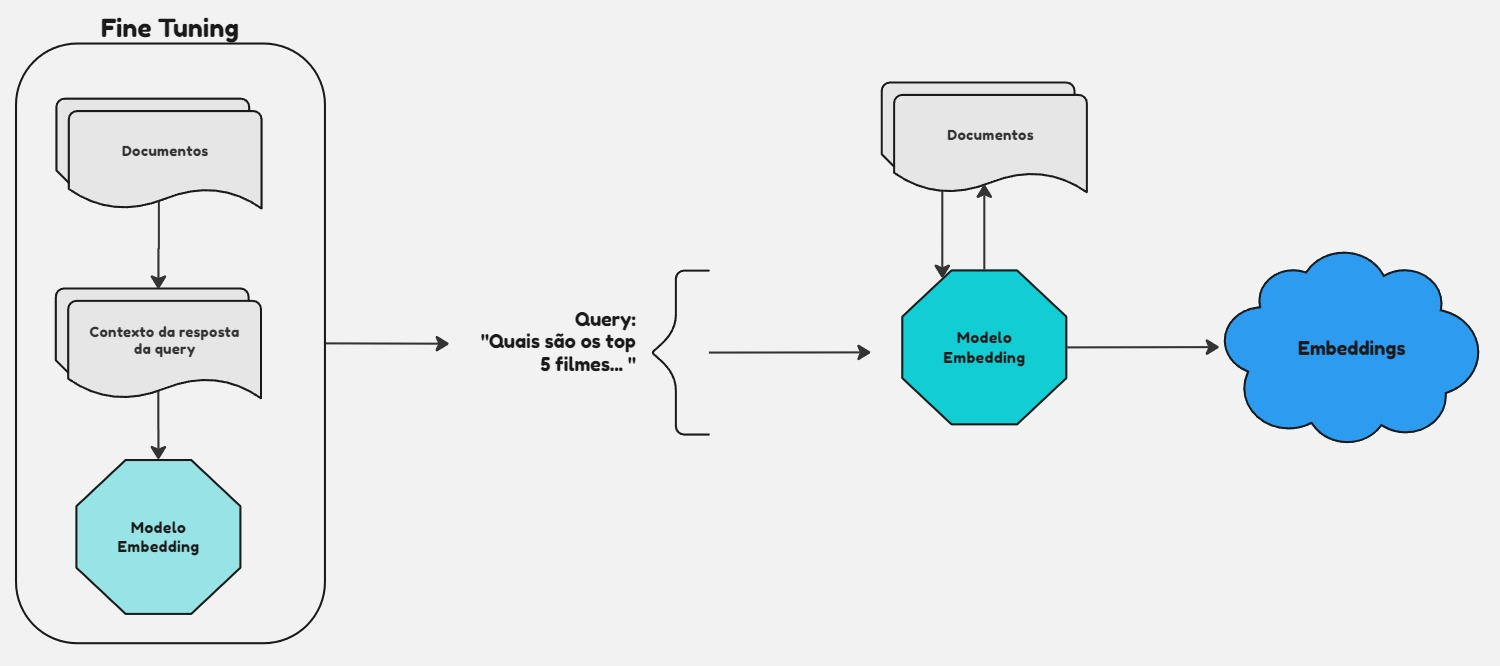
\includegraphics[width=\linewidth]{img/retrieval2.jpg}
    \caption*{Fonte: Do Autor}
    \label{fig:retrieval2}
\end{figure}

\subsection{\textit{Generation}}

A etapa de Generation consiste em receber as informações recebidas na etapa de Retrieval, e transformá-las em texto fluente. Os dados recuperados, \textit{embeddings}, sao incorporados no modelo LLM que é capaz de retornar o texto mediante o contexto. O texto gerado contempla informações tanto dos novos documentos recebidos como contexto, quanto dos dados previamente existentes e pré-treinados do proprio modelo. Modelos como BERT \cite{alaparthi2020bidirectionalencoderrepresentationstransformers} e LLama \cite{llama3modelcard} mencionados nos capítulos \ref{bert} e \ref{llama} são responsaveis por gerar o texto, recebendo os documentos mais relevantes dado a \textit{query}.


\subsection{\textit{Vector} RAG vs \textit{Graph} RAG}

Os bancos de dados vetoriais se destacam no armazenamento e gerenciamento de dados não estruturados, como textos, imagens e áudios, convertendo-os em \textit{embeddings} vetoriais. Esses \textit{embeddings} capturam as relações semânticas entre os pontos de dados, permitindo buscas de similaridade rápidas e eficientes. Quando um sistema RAG consulta um banco de dados vetorial, ele identifica rapidamente vetores matematicamente próximos, calculado por uma distância euclidiana, por exemplo \cite{DANIELSSON1980227}  que deveriam implicar significados semelhantes, em vez de depender apenas da correspondência de palavras-chave.

\subsubsection{Vantagens de aplicação do contexto vetorial}
Essa capacidade é especialmente favoravel a contextos de RAG, onde a compreensão e a interpretação do contexto são cruciais. A identificação de similaridades semânticas pode proporcionar recomendações mais precisas e relevantes. Além disso, em algoritmos de busca ou modelos de \textit{embeddings}, essa abordagem permite recuperar informações mais pertinentes, melhorando a experiência do usuário ao fornecer resultados que realmente correspondem à intenção da consulta. Portanto, os bancos de dados vetoriais oferecem uma vantagem significativa na manipulação de grandes volumes de dados não estruturados, garantindo eficiência e precisão na recuperação da informação.

 A Figura \ref{fig:vector_db} é representada pelas consultas a partir de uma \textit{query}, no contexto de \textit{Vector Databases}. Dado uma \textit{query} de entrada e um conteúdo de documentos (\textit{content}), esses valores passam pelo modelo de \textit{embedding} (\textit{embedding model}) e retorna um vetor dimensional com similaridade de cada documento dado a \textit{query} de entrada, esses vetores pré-gerados são armazenados em uma base de dados vetorial que será posteriormente utilizado para consulta de RAG.

\begin{figure}[!htb]
    \centering
    \caption{Recuperação baseada em \textit{Vector databases}.}
    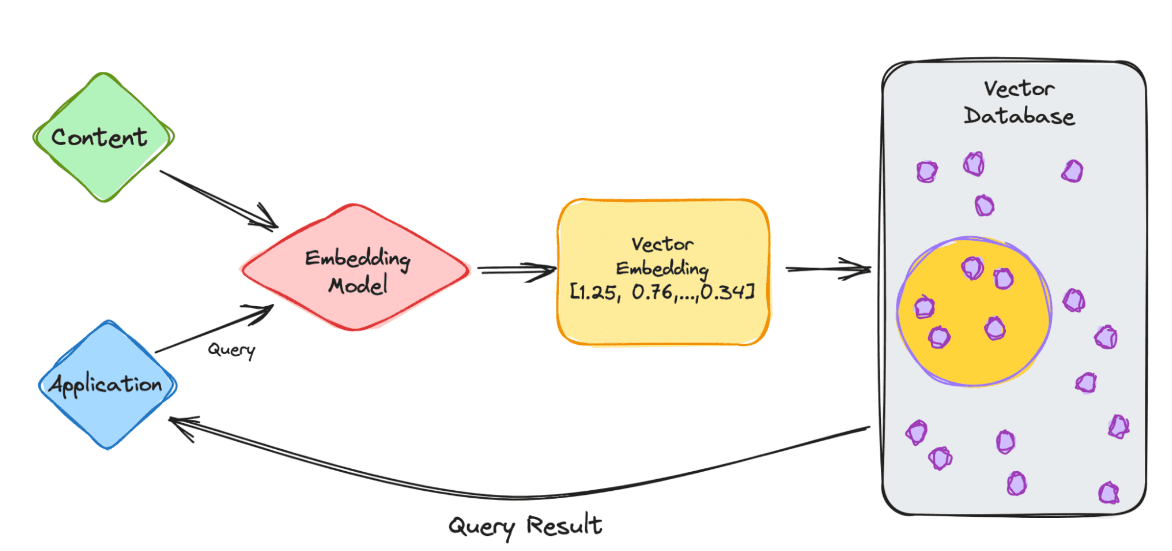
\includegraphics[width=\linewidth]{img/vector_db.png}
    \caption*{Fonte: kdnuggets}
    \label{fig:vector_db}
\end{figure}

\subsubsection{Limitações do contexto vetorial}
No entanto, os bancos de dados vetoriais têm algumas limitações quanto ao contexto RAG. Eles podem enfrentar dificuldades com consultas complexas que exigem uma compreensão profunda das relações e dependências entre entidades. Além disso, o processo de conversão de dados em \textit{embeddings} vetoriais pode levar à perda de contexto e nuances, o que pode afetar a precisão e a explicabilidade das respostas geradas \cite{kang2024promptragpioneeringvectorembeddingfree}. Embora os \textit{embeddings} vetoriais capturem relações semânticas, nem sempre conseguem representar todas as interdependências detalhadas e específicas entre os dados. Isso é particularmente problemático em domínios que exigem alta precisão e clareza nas relações.

A perda de contexto e nuances ocorre porque o processo de vetorização simplifica a informação em uma representação matemática. Durante essa simplificação, detalhes sutis e contextuais podem ser omitidos, resultando em uma representação que, embora útil, não é perfeita. Isso pode levar a respostas que, apesar de aproximadas, carecem de uma explicação clara sobre como foram derivadas, dificultando a compreensão completa da lógica por trás dos resultados \cite{cheng2024characterizing}.

\subsubsection{Grafos de conhecimento em RAG}
O Graph RAG utiliza um grafo de conhecimento, equiparando-o a um vocabulário em larga escala onde entidades e relacionamentos correspondem a palavras. Isso permite a modelagem conjunta de entidades e relacionamentos durante a recuperação de informações, o que aprimora a compreensão da intenção da consulta e fornece resultados de busca mais precisos \cite{edge2024local}.

Diferente dos bancos de dados vetoriais, os grafos de conhecimento representam dados como uma rede de nós (entidades) e arestas (relacionamentos). Essa estrutura captura relações e dependências complexas, permitindo consultas semanticamente entrelaçadas que exigem um entendimento profundo do contexto dos dados. Os grafos de conhecimento são particularmente eficazes para compreender não apenas um ponto de dado isolado, mas suas relações e o contexto mais amplo. Eles usam o modelo de triplas semânticas, codificando informações como expressões sujeito-predicado-objeto (por exemplo, "Pedro joga \textit{league of legends}" ou "Pedro vai pra academia"), o que mantém a fidelidade dos dados durante a recuperação e permite um rastreamento robusto. A Figura \ref{fig:rag5} representa um Grafo de conhecimento.

\begin{figure}[H]
    \centering
      \caption{Grafo de conhecimento representado por nós (entidades) e arestas (relacionamentos).}
    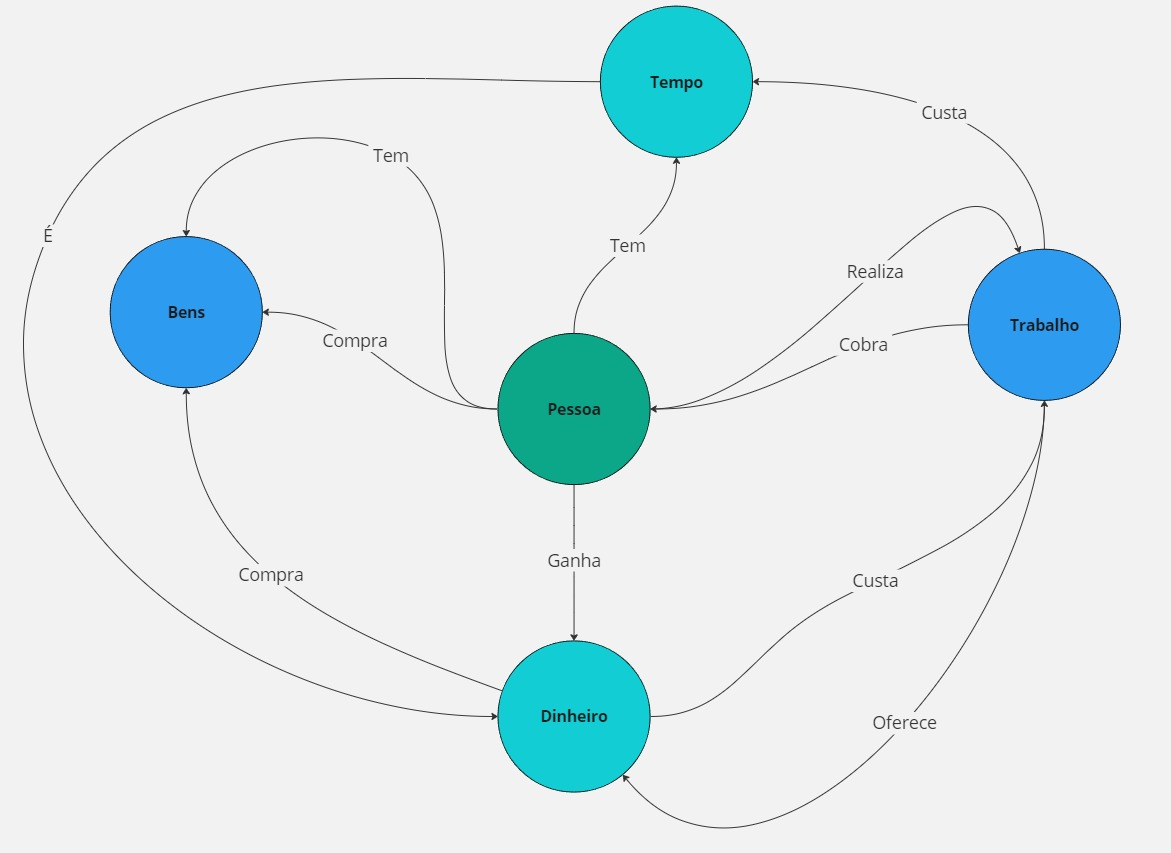
\includegraphics[width=\linewidth]{img/rag5.jpg}
    \caption*{Fonte: Do Autor}
    \label{fig:rag5}
\end{figure}


\subsubsection{Vantagens e desvantagens dos grafos de conhecimento em RAG}
Uma vantagem chave dos grafos de conhecimento é a explicabilidade. Relacionamentos explicitamente definidos permitem que o sistema RAG rastreie o caminho seguido para chegar a uma resposta, aumentando a transparência e a confiança. Isso torna os grafos de conhecimento bem adequados para aplicações que exigem raciocínio complexo e inferência, como sistemas de perguntas e respostas ou ferramentas de suporte à decisão.

Entretanto, a complexidade de estruturar um grafo de informação aumenta, tornando o processo mais complexo. Além disso o Graph RAG pode enfrentar quedas de desempenho em conjunto de dados grandes.



\subsection{\textit{Fine Tuning} vs RAG}

De acordo com \cite{gao2024retrievalaugmentedgenerationlargelanguage}, existe uma diferença de decisão diante da escolha do melhor caminho a seguir quanto à implementação de modelos de geração de texto usando LLM. Existem abordagens e contextos das quais fazem sentido efetuar um Fine Tuning no modelo previamente treinado, para o objetivo específico, ou implementar um fluxo de RAG para retornar o conteúdo mais relevante dado uma entrada.

As principais diferenças se dão pelo fato de que o \textit{fine tuning} se comporta como um aprendizado adicional, que é internalizado, um conhecimento que é estático e adicionado ao modelo. Para isso é necessaria uma base de conhecimento, estruturada e carregada de acordo com as exigências de entrada do modelo escolhido. 

Já o RAG, é o metodo que tem a premissa de buscar os documentos mais relevantes para a \textit{query} de entrada, e, a partir disso, atribuir como insumo pontual do modelo para retornar o texto contextualizado.

As principais diferenças se dão pelos elementos a seguir, de acordo com \cite{gao2024retrievalaugmentedgenerationlargelanguage}.

\subsubsection{Conhecimento do modelo}
\label{knowledge}
A vantagem do RAG em relação ao ganho de conhecimento, é a etapa baseada no \textit{Retrieval}, que a informação atual de um determinado contexto é utilizada como retorno para o escopo da resposta, sem precisar realizar re-treinos no modelo, o que o torna mais flexível e com maior adaptabilidade à mudanças de conteúdo da informação, seja de fontes externas ou dados não estruturados. Por sua vez, o \textit{fine tuning} requer uma base estruturada com a necessidade de realizar um treinamento com as novas informações, gerando o custo de tempo e recursos computacionais.

\subsubsection{Processamento de dados}
\label{dataprocess}
Para o RAG, existe um mínimo de processamento de dados, pelo tratamento e organização dos documentos nas bases vetoriais, realizar a indexação e um tratamento prévio quando cabível. No \textit{fine tuning}, é necessario ter o conjunto de dados em um alto nível de qualidade para servir como \textit{input} para o treinamento do modelo, devem ser realizadas adaptações nos dados para a necessidade de parâmetros, o que o torna essa etapa mais complexa e demorada. 

\subsubsection{Modelagem}
\label{modeling}
Para entregar respostas customizadas, no \textit{fine tuning} é possivel customizar as perguntas e respostas, colocar o modelo para reagir de forma especifica a uma determinada pergunta, o que o torna vantajoso para cenários de adaptações específicas. No RAG, como é focado em retornar informações dados relevantes de fontes não incorporadas no modelo, não é possível customizar de forma assertiva o resultado ou a forma de escrita das respostas.

\subsubsection{Recursos computacionais}
\label{resources}
Para retornar os dados mais relevantes no contexto RAG, dependendo da estratégia de retorno, pode-se exigir um maior recurso computacional em cada inferência, e existe também a necessidade de manter as fontes externas atualizadas e organizadas. No \textit{fine tuning} existe a necessidade de realizar o tratamento e preparação dos dados, a etapa de treinamento, exerce um alto recurso pontual no processamento paralelo em GPU/TPU.

\subsubsection{Latência}
\label{latency}
No RAG, pelo fato de existir um processamento de dados na etapa de \textit{Retrieval}, a latência é maior para cada inferência individual do modelo, dependendo da estratégia de ranqueamento, armazenamento e indexação, podendo ocorrer um tempo longo de retorno da consulta. A vantagem do \textit{fine tuning} nesse aspecto é a velocidade da inferência, como o modelo já está treinado e detém do conhecimento previamente fornecido ao modelo, o tempo de resposta é menor.

\subsubsection{Alucinações}
\label{alucinations}
O RAG detém de uma menor chance de obter alucinações em comparação ao \textit{fine tuning}, pelo fato de que os documentos são retornados de um contexto de domínio especifico, quando encontrados. Para trabalhar na redução de alucinações no \textit{fine tuning}, é necessário treinar o modelo baseado em conjuntos de dados específicos.